\label{chap:methodical_approach}

The goal for the developed workflow is to identify several approaches and sub-steps for the automated extraction of semantically linked metadata.
As a first overview of the workflow, \cref{fig:workflow-concept} shows the steps on a conceptual level.
It starts with the input of a dataset.
Those datasets are not manually adjusted before being fed into the automated extraction process, so that the methodology imposes no specific requirements other than the presence of text-based, decodable files.
After that, the files are preprocessed before they are split into smaller chunks.
At the same time, a dataset-level context overview is generated based on the dataset structure and per-file summaries.

With the help of the generated context, the individual chunks are processed by an \ac{LLM} to extract metadata signals.
Those signals are not yet interpreted in the context of a specific metadata profile, but serve as an intermediate representation of the extracted information.
This follows the \ac{GO} approach, where the extraction of information is separated from the organization of that information into a specific schema to reduce the cognitive load \cite{li2024structuredoutput}.
As soon as the process finishes with the chunk iteration, the extracted signals are merged and deduplicated to form the evidence grounding set for the next steps.
After the grounding set is in place, a \ac{DCAT-AP+} artifact is initialized to serve as the target schema for the extracted information.
In order to fill the schema, the workflow follows a requirement-driven approach, where the schema is iteratively checked for missing information and the missing information is extracted from the evidence grounding set.
If a requirement cannot be fulfilled, it is flagged for manual curation.
Once that is done, the workflow continues with the final step of running queries against a property graph of controlled vocabularies.
This allows a mapping of \texttt{DefinedTerms} shapes from the \ac{DCAT-AP+} artifacts to suitable concepts and classes via \texttt{dcterms:type} or \texttt{rdf:type}.

\begin{figure}[H]
    \centering
    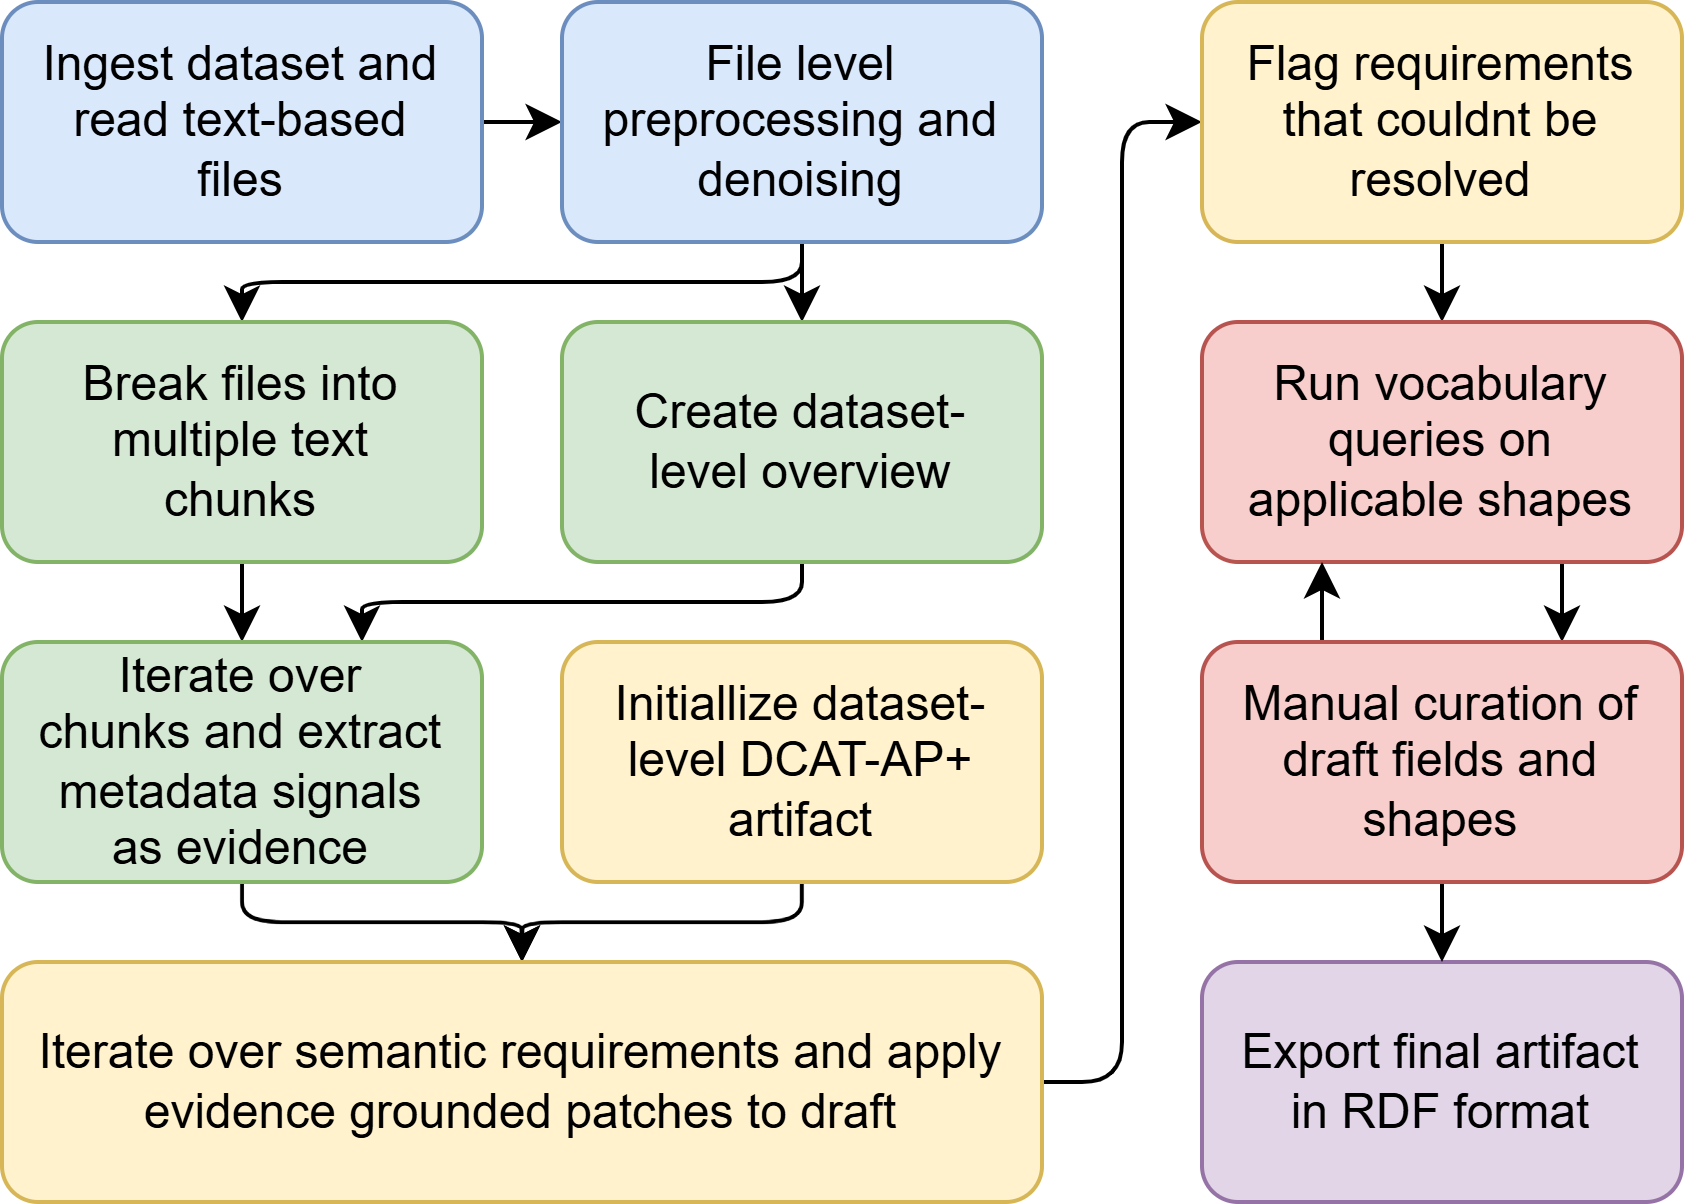
\includegraphics[height=0.3\textheight]{figures/workflow-concept.png}
    \caption{Conceptual overview of the workflow}
    \label{fig:workflow-concept}
\end{figure}


\section{Datasets}
\label{sec:datasets}

The workflow has been designed to be applicable to any type of dataset that contains text-based files.
Therefore, it is not limited to a specific field or file format.
This study used a number of \ac{NMR} datasets as test datasets.
One sample is first presented below to provide an overview of the resources these datasets contain.

The sample dataset consists of a single one-dimensional \textsuperscript{1}H NMR dataset exported from ChemSpectra, a web-based spectra editor for analytical data \cite{Huang2021}.
\Cref{fig:1H-NMR-dataset} shows the dataset structure and its contents.
Within this export, the nested archive \texttt{10.zip} preserves the native Bruker instrument output and is therefore treated as an example for a raw instrument generated input for the metadata-extraction workflow.
The archive contains the acquired \ac{FID} signal together with the associated acquisition parameters.
In contrast, the accompanying files generated by ChemSpectra represent a standardized spectral representation.
Using both the raw and standardized files as input allows the workflow to be evaluated on both types of data, which are expected to be present in real-world datasets.

\begin{figure}[H]
    \centering
    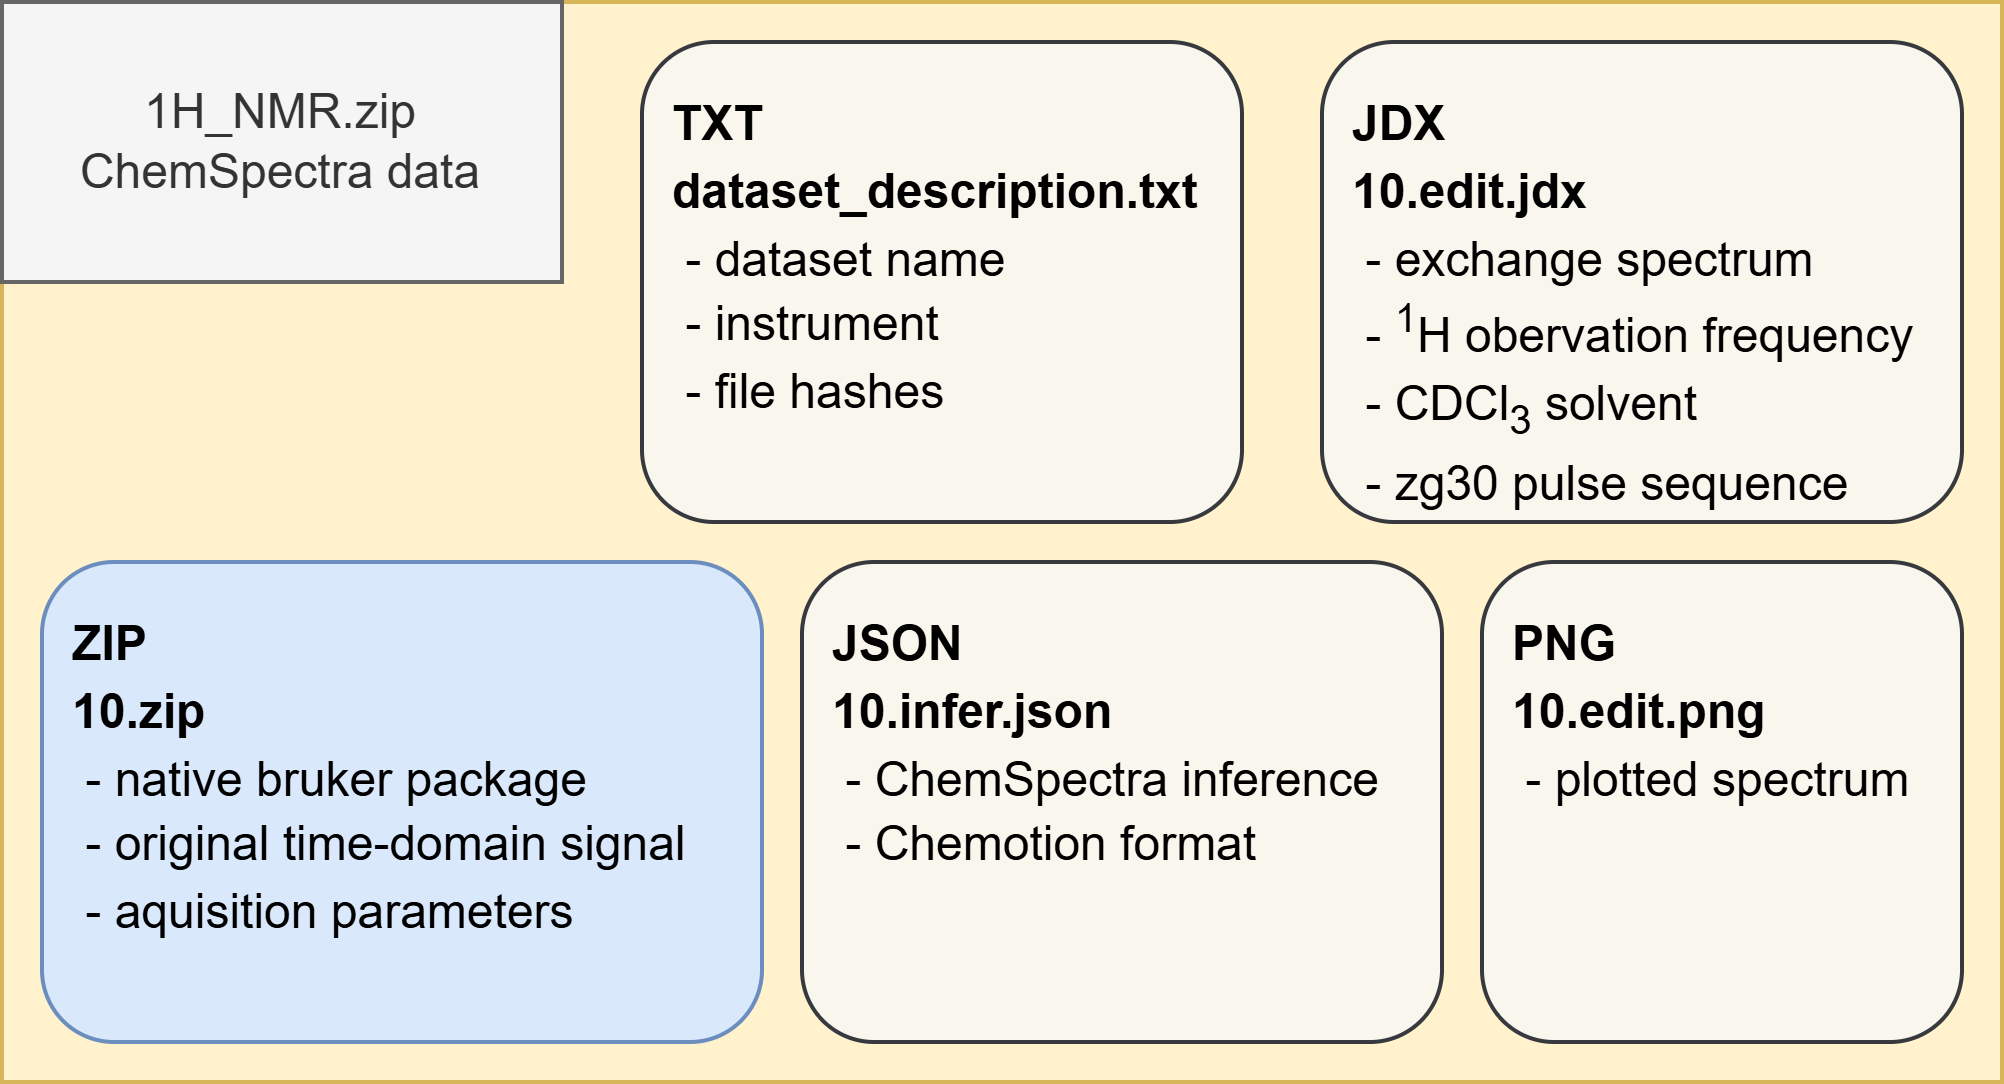
\includegraphics[width=0.8\textwidth]{figures/1H-NMR-dataset.png}
    \caption{Sample \textsuperscript{1}H NMR dataset with its file contents.}
    \label{fig:1H-NMR-dataset}
\end{figure}

